\documentclass[f,bachelor,binding,twoside,palatino]{WeSTthesis}
% Please read the README.md file for additional information on the parameters and overall usage of WeSTthesis

\usepackage[ngerman, english]{babel}         % English and new German spelling
\usepackage[utf8]{inputenc}                 % correct input encoding
\usepackage[T1]{fontenc}                    % correct output encoding
\usepackage{graphicx}                       % enhanced support for graphics
\usepackage{tabularx}                       % more flexible tabular
\usepackage{amsfonts}                       % math fonts
\usepackage{amssymb}                        % math symbols
\usepackage{amsmath}                        % overall enhancements to math environment
\usepackage[babel,english=british]{csquotes}
\usepackage{enumitem}
\usepackage{url}
\usepackage{glossaries}
\usepackage{xcolor}
\usepackage{float}
\makeglossaries

\def \ajax {AJAX}
\def \pjaxr {PJAXR}
\def \jqueryPjaxr {jquery-pjaxr}
\def \djangoPjaxr {django-pjaxr}
\def \phpPjaxr {php-pjaxr}
\def \httpRequest {HTTP request}
\def \singlePageApplication {single-page application}
\def \SinglePageApplication {Single-page application}

\usepackage{glossaries}

\newglossaryentry{ajax}
{
  name=AJAX,
  description={Asynchronous JavaScript and XML \footnote{\url{https://developer.mozilla.org/de/docs/AJAX}}}
}

\newglossaryentry{djangoLare}
{
  name=django-lare,
  description={The \lare{} backend for django}
}

\newglossaryentry{dynamicWebPage}
{
  name=dynamic web page,  
  description={A dynamic web page is a web page that is generated by a web application on a web server before it gets delivered.}
}

\newglossaryentry{hijax}
{
  name=HIJAX,
  description={Hijax}
}

\newglossaryentry{html}
{
  name=HTML,
  description={HTML stands for Hyper Text Markup Language and is the language that is used in the Web.}
}

\newglossaryentry{httpRequest}
{
  name=HTTP request,
  description={Hypertext Transfer Protocol requests build the foundation for data communication in the World Wide Web.}
}

\newglossaryentry{lareJS}
{
  name=lare.js,
  description={lare.js is the \lare{} frontend and the \ajax{} engine for \lare{}.}
}

\newglossaryentry{phpLare}
{
  name=PHP-lare,
  description={PHP-lare is the \lare{} backend for PHP.}
}

\newglossaryentry{lare}
{
  name=Lare,
  description={Lightweight asynchronous replacement engine is a technology for stateful \singlePageApplication{}s.
  It consists of a \lare{} frontend as ajax engine, and a \lare{} backend which is plugged into the web application.}
}

\newglossaryentry{singlePageApplication}
{
  name=single-page application,
  description={A single-page application is a web application or web site that retrieves one full \webPage{}.
  Beside this first page load, the web site is not loaded completely at any point in the process anymore.
  Often content changes are made asynchronous and dynamically by \ajax{} in response to user actions.}
}

\newglossaryentry{staticWebPage}
{
  name=static web page,
  description={A static web page is a web page that is delivered exactly as stored in the web server's file system.}
}

\newglossaryentry{twig}
{
  name=Twig,
  description={Twig}
}

\newglossaryentry{twigLare}
{
  name=Twig-lare,
  description={Twig-lare is the \lare{} backend for Twig and uses \phpLare{}.}
}

\newglossaryentry{url}
{
  name=URL,
  description={A Uniform Resource Locator identifies and defines the location of a resource, e.g. a \webPage{}.}
}

\newglossaryentry{w3c}
{
  name=W3C,
  description={The World Wide Web Consortium (W3C) is an international community where Member organizations, a full-time staff, and the public work together to develop Web standards. Led by Web inventor Tim Berners-Lee and CEO Jeffrey Jaffe, W3C's mission is to lead the Web to its full potential.\footnote{http://www.w3.org/Consortium/}}
}

\newglossaryentry{webApplication}
{
  name=web application,
  description={A web application is a application that generates \webPage{}s.}
}

\newglossaryentry{webPage}
{
  name=web page,
  description={A web page is a single document and part of a web site. 
  Every page should be accessible over the Internet and has it's own URL.
  A web browser can retrieve web pages by making \httpRequest{}s and it can render them afterwards.}
}

\newglossaryentry{webSite}
{
  name=web site,
  description={A web site is a collection of \webPage{}s that are linked to each other.}
}



\author{Jonas Braun}

\title{\pjaxr{} - A new technology for stateful \singlePageApplication{}s}

\degreecourse{Computervisualistik}

\firstreviewer{Prof. Dr. Steffen Staab}
\firstreviewerinfo{Institute for Web Science and Technologies}

\secondreviewer{René Pickhardt}
\secondreviewerinfo{Institute for Web Science and Technologies}


\begin{document}

% optional: change document language from ngerman to english
% \selectlanguage{english}

\maketitle %prints the cover page  an empty page if two-sided print
\pagenumbering{roman}

\tableofcontents

\varclearpage

% list of figures
% \listoffigures
% \varclearpage

\pagenumbering{arabic}

% beginning of the actual text section
\newcommand\todo[1]{\textcolor{red}{#1}}

\section{Introduction}
  At the beginning of the World Wide Web websites were self-contained. The content which was initially loaded was not changed until a new URL was requested by the user.
  One big change was the invention of \ajax{}. It introduced the possibility to change content without the need of requesting a new URL.
  This approach only loading one website initially and then changing its content interactively is called \singlePageApplication{}.
  \SinglePageApplication{}s are more user-friendly than the common designs, e.g. due to lower load times in combination of not being able to indicate clearly that a new website is being loaded.
  A big disadvantage of those are that users are not able to save their websites as a bookmark, because while surfing on this page, the URL never changes.
  This technique is available in nearly every browser which is a reason that a lot of different frameworks gain this functionality, improving and enhancing it.

  \SinglePageApplication{}s have a problem in the current time: Search engines and other crawlers trying to examine websites will find nothing more than content which was provided initially. Every further change of content is not easily accessible.
  As Google is the most used search engine in the World Wide Web they have a design pattern\footnote{https://developers.google.com/webmasters/ajax-crawling/docs/getting-started} for implementing a crawlable \ajax{} web application. 
  In this guideline it is recommended to have snapshots available under non-user-friendly URLs, called Hash-Bang URLs.

  In this thesis we will improve and evaluate a new technology called \pjaxr{}. 
  Together with Stephan Groß we developed this technique for using \ajax{} with it's advantages but trying to avoid the disadvantages explained before.
  The result of that cooperation is the frontend-side implementation called \emph{\jqueryPjaxr{}}.
  As \pjaxr{} also needs a backend to be implemented, we developed the first \pjaxr{} backend called \emph{\djangoPjaxr{}}.
  Additionally in this thesis we will introduce a new \pjaxr{} backend for PHP, \emph{\phpPjaxr{}}.
  
  
\section{Fundamentals}
  To understand how \ajax{} and similar techniques work, you have to understand how \httpRequest{}s work:
  First a browser interprets the URL and requests the path, e.g. "/index.html" from the host, e.g. "google.de" via the protocol, e.g. "http".
  Then the webserver analyses the request and responds with the content, corresponding to the requested path.
  To display the requested website, the browser interprets the response and renders the content. 
  Images, JavaScripts and Stylesheets which are linked inside the response are retrieved and interpreted the same way on further \httpRequest{}s.

  The first response is typically a HTML file.
  Starting with the used document type those files have a XML like structured hierarchy.
  Every item inside is a semantic tag, which can have attributes like a class or an ID.

  \SinglePageApplication{}s using \ajax{} aim on changing those tags dynamically without having to load a full new page.
  When e.g. clicking a link JavaScript will prevent the default browser functionality. Instead it requests a special URL to retrieve some data, most often JSON, which is then interpreted and rendered.

  Introducing HTML 5 on 28th October 2014 W3C released a new standard for HTML and associated APIs. 
  This release introduced officially the History API.

\section{State of the art}
  \ajax{} is a widely used technique in the internet to build web applications because of the UX improvements it brings.
  In \cite{roodt06} is mentioned that \ajax{} applications have a better usability than non-\ajax{} websites.
  The same conclusion is made in \cite{klugeKarglWeber07}, despite of the lack of browser navigation support.
  Beside the navigation problem another disadvantage is, as presented in \cite{mesbah09}, crawling \ajax{} applications is not trivial.
  One solution of this task is finding clickables and navigating to every page found by this.
  Nevertheless \cite{mesbah09} states also that this only generates a snapshot of the full application.
  This difficulty of crawling those websites is additionally presented by search engines, avoiding this problem.\cite{matter08}, page 81
  Currently the task of building a crawlable \singlePageApplication{} using \ajax{} is often being avoided, instead crawling algorithms are getting improved and in focus of research.

  A common way to implement \ajax{} in websites is to use the pattern of HIJAX.
  It says to plan with \ajax{} from the start of building the website but build it without and after the website is finished without \ajax{} you add it afterwards.
  This should then be done by \emph{hijacking} an event like a click to then handle it by an additional script.

  
\section{\pjaxr{}}
  \subsection{Requirements}
  The idea of \pjaxr{} is to have the advantages of \ajax{} while trying to avoid it's disadvantages.
  This means it should have the same UX improvements, and reduced load times as classical \ajax{}.
  On the other hand \singlePageApplication{}s using \pjaxr{} should be easily crawlable by the most used crawlers without additional efforts.
  E.g. it should not be necessary to have several endpoints with the same content for crawlers and normal users.
  Additionally \pjaxr{} should be a generic solution for \singlePageApplication{}s, not just for one specific.

  \subsection{Concept}

  \begin{figure}[H]
    \centering
    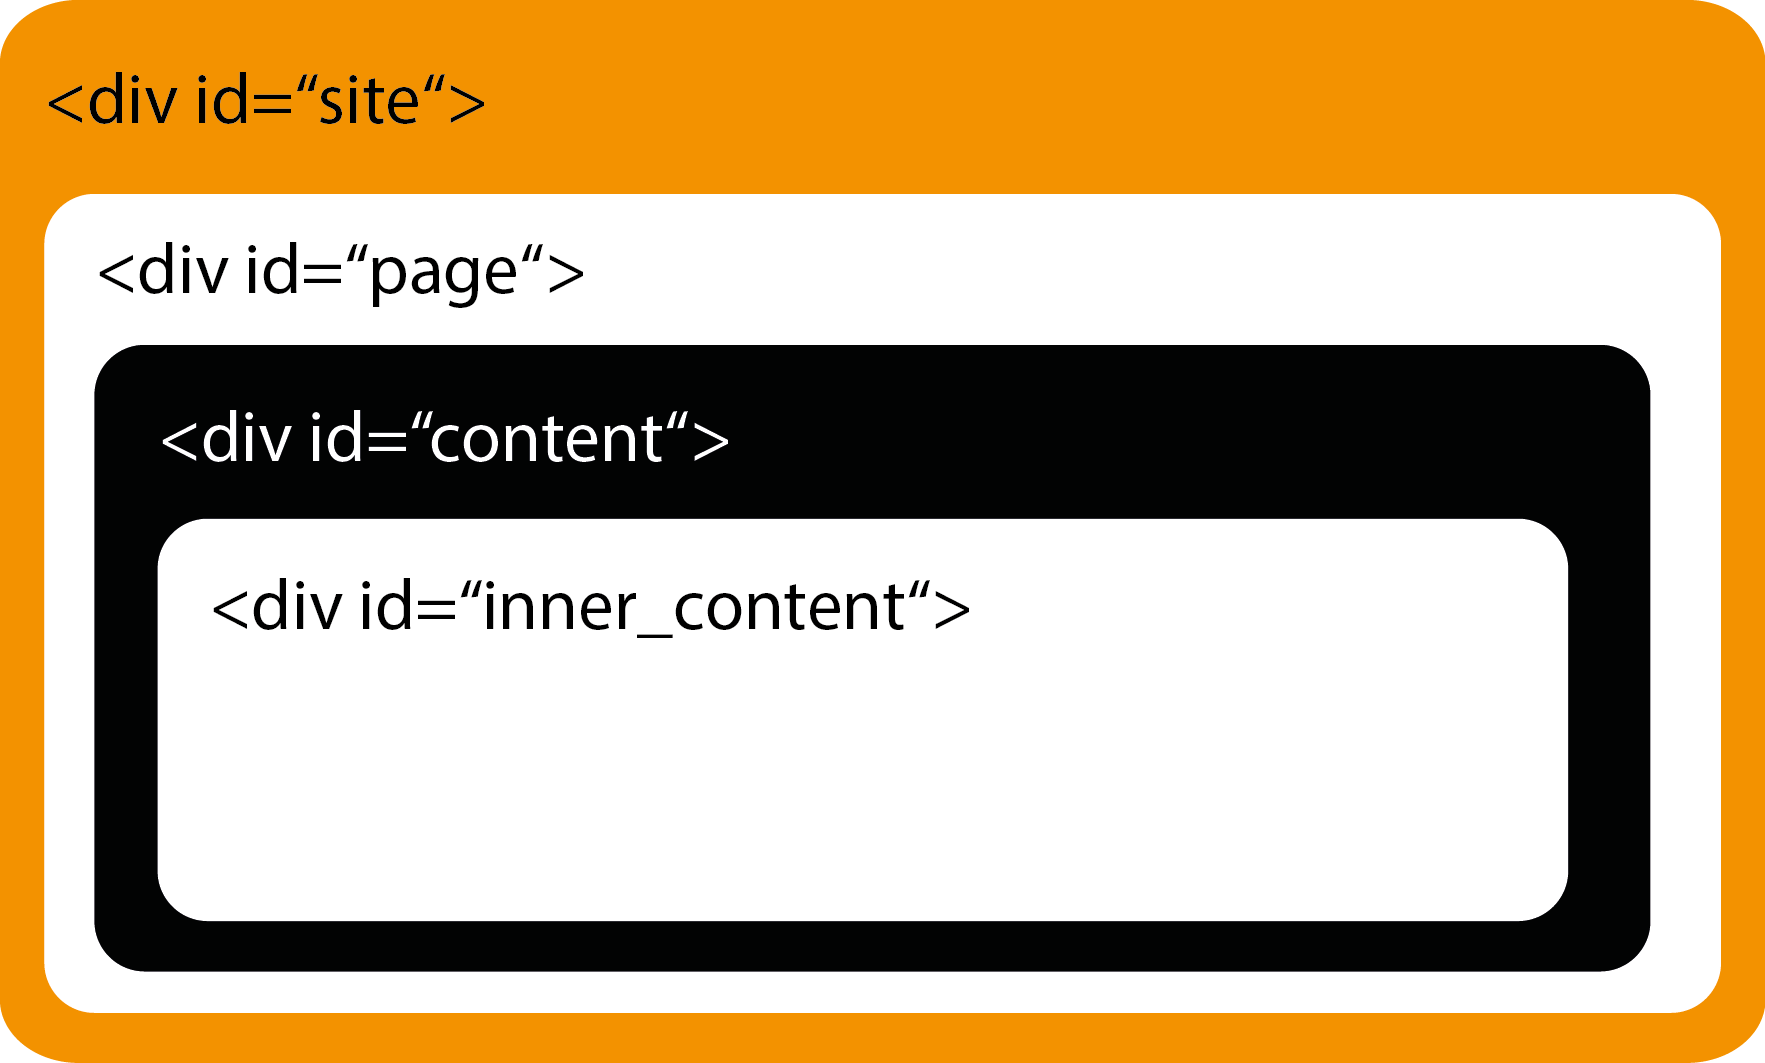
\includegraphics[width=13cm]{images/pjaxr_html.png}
    \caption[pjaxr_html]{Basic HTML structure of a web application using \pjaxr{}}
    \label{fig:pjaxr_html}
  \end{figure}

  Every \singlePageApplication{} which uses \pjaxr{} has a hierachically namespace structure.
  Typically the namespace consists of a prefix, a site id, a page id, a content id and an inner-content id.
  Every level in the hierarchy has it's counterpart on the website as shown in figure \ref{fig:pjaxr_html}, a container with an id telling which part of the namespace it belongs to.
  After the \pjaxr frontend is initialized it hijacks events like clicks on links and enriches the request with the current website's namespace.
  A \pjaxr{} backend analyzes the namespace of the requested website and the one sent in the request.
  The most top-level part of the namespaces not matching is the decisive one.
  The containers according to this namespace will be responded to the request.
  An optimized web application should only grab the necessary data and render it afterwards.
  The \pjaxr{} frontend retrieves the response and replaces the according containers at the website and updates the the current namespace.
  
  \begin{figure}[H]
    \centering
    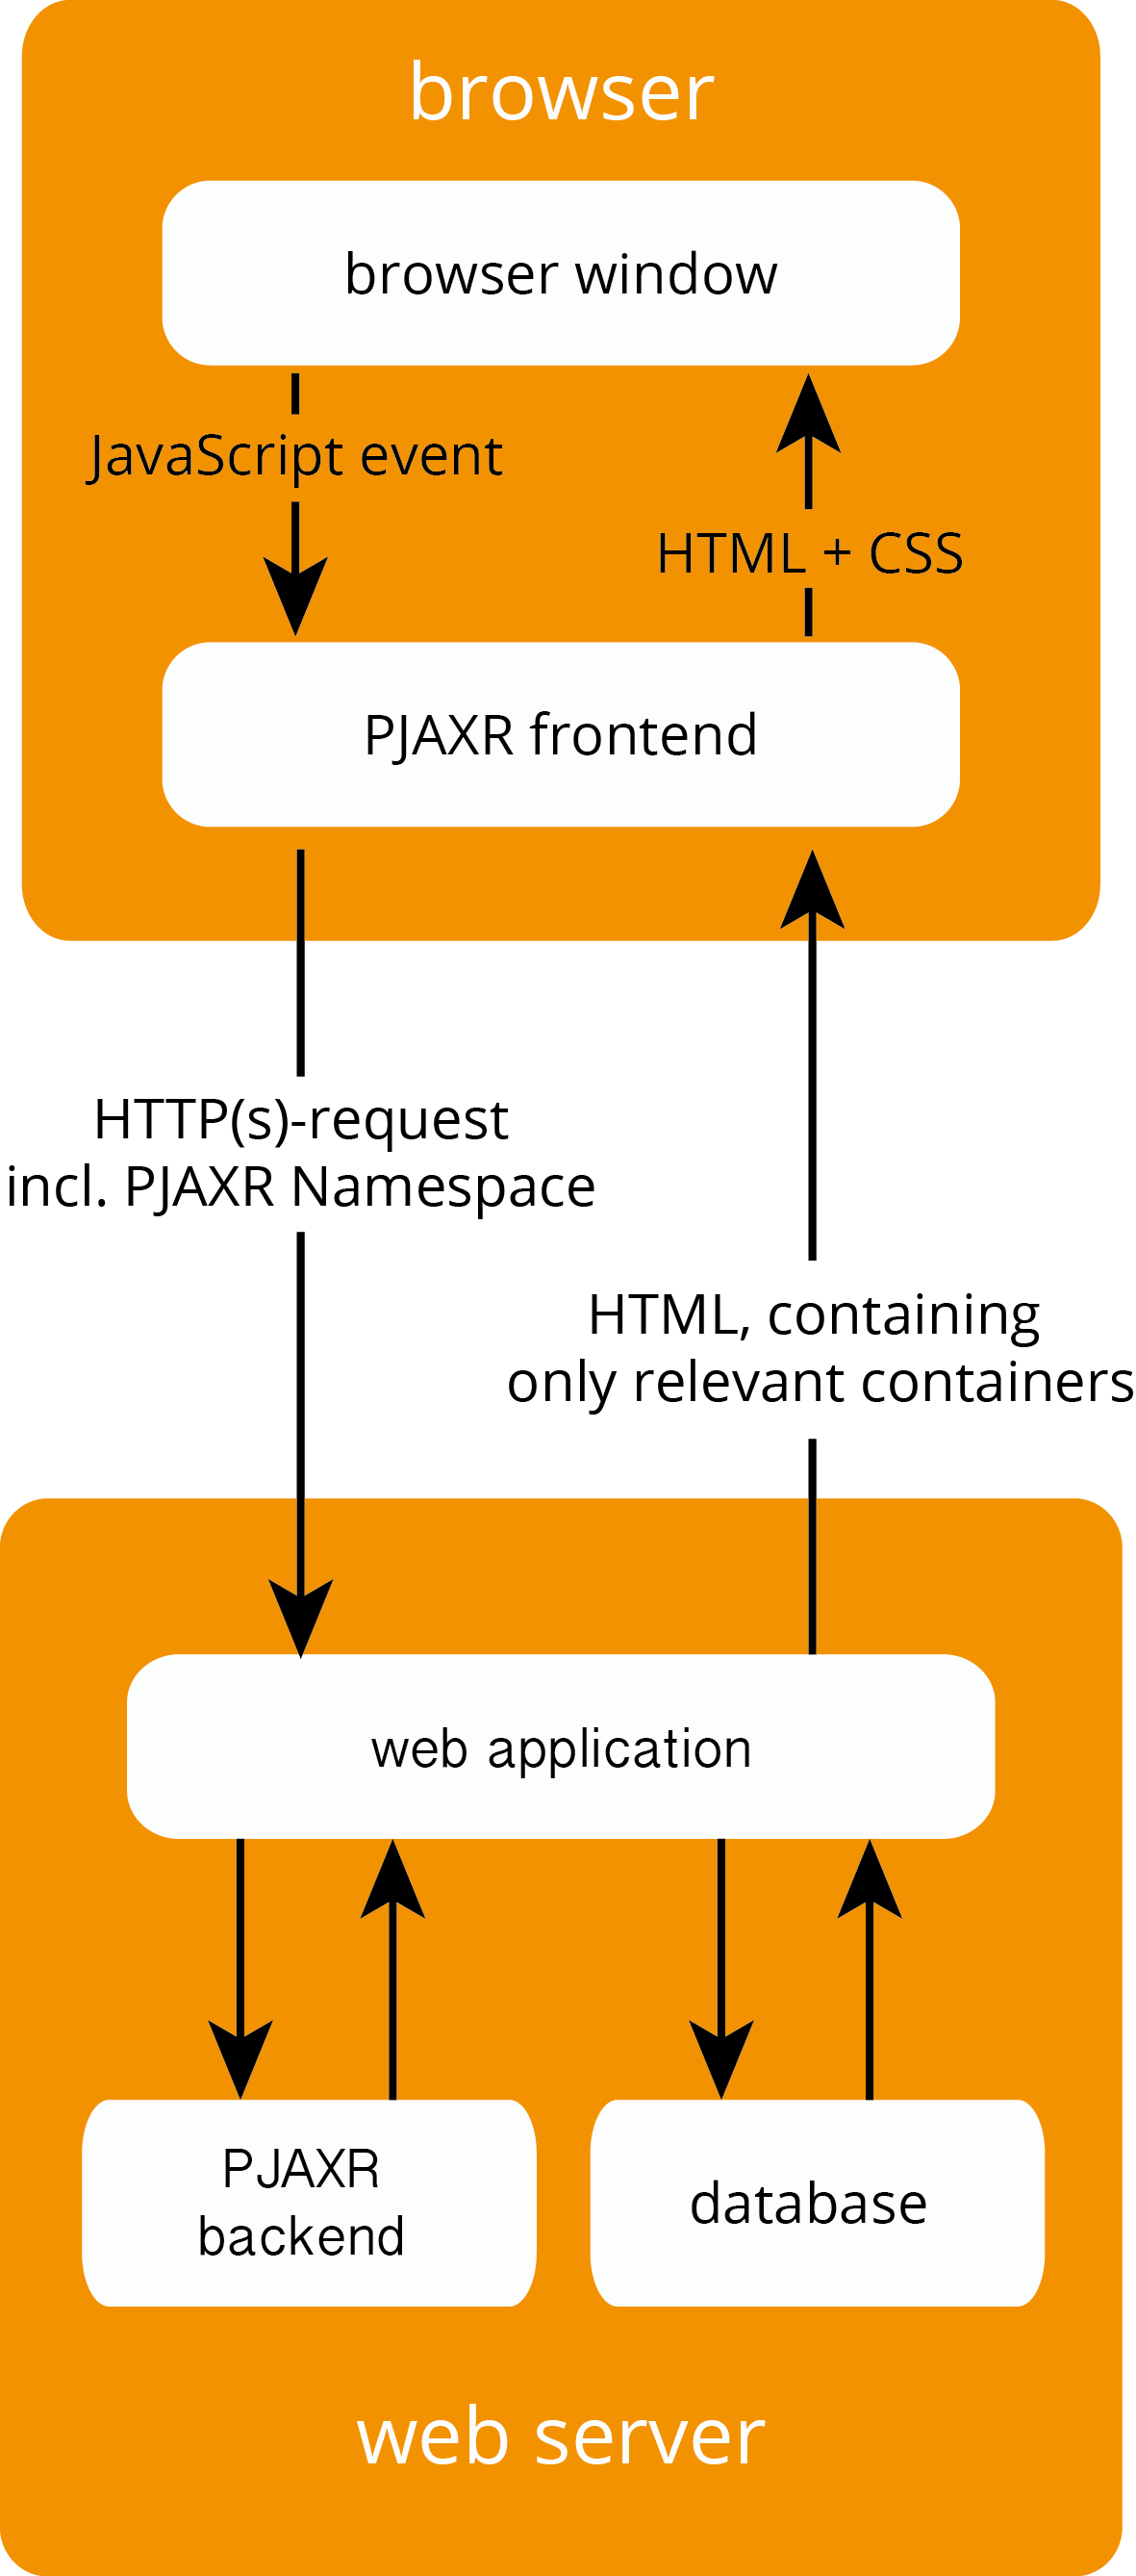
\includegraphics[height=10cm]{images/pjaxr.png}
    \caption[pjaxr_components]{Component and communication diagram of \pjaxr{}}
  \end{figure}
  
  \subsection{Realization}
  To load a page, the first request is a normal \httpRequest{} followed by a JavaScript initializing the \pjaxr{} frontend module.
  Further requests to the same host are then initated by this module.
  The HTTP header of those requests are extended by the namespace of the current website.
  The webserver using a \pjaxr{} backend detects the first namespace of the requested resource not matching the namespace of the HTTP header.
  It then decides which data is needed to be gathered and which template should be used to render those.
  The content delivered by the \pjaxr{} backend enriched web server is interpreted by the frontend module and replaces the related containers.
  This replacement is implemented using the ID attribute.
  Other methods identifying corresponding containers like e.g. the XPath are not as generic in it's position on the page as the ID.
  This is important because \singlePageApplication{}s should be able to include content dynamically in every position on the page.
  \pjaxr{} in combination with the History API makes it then possible to update the content and change the URL like it would be made by normal requests.
  This is possible with the use of the pushState method introduced in the History API.
  Back- and forward-buttons and bookmarks in a browser will work as it were a normal request using this function.
  
\section{Implementation}
  Part of the thesis is to evaluate \pjaxr{}. For that reason a sample web application will be implemented, which will provide non-\ajax{}, \ajax{}-based and \pjaxr{}-based endpoints.
  This will especially include an implementation of a \pjaxr{} backend for PHP. As another part \jqueryPjaxr{}, the \pjaxr{} frontend module will be adjusted to fulfil the requirements for a PHP backend.

\section{Evaluation}
  As one traditional testing model, we will evaluate the \pjaxr{} sample application via blackbox tests.
  Testing \ajax{} is not trivial due to multiple programming- and markup-languages influencing it. 
  One possibility to test web applications, as suggested in \cite{lundmark11}, is Selenium\footnote{http://www.seleniumhq.org/}.
  With this tool it is possible to generate automated tests for web applications.

  To evaluate whether the application is crawlable or not is an important criteria whether \pjaxr{} fulfills it goals.
  Finding all the content delivered in all different URLs in the sitemap should be the target to acquire.
  The crawled content should be similar to a non-dynamic HTML file, defined for every URL.
  Content which is not directly provided via an URL but asynchronously, like via an autocompletion, should not be relevant.

  One way to crawl \ajax{} web applications, recommended in \cite{crawljax:tweb12} is to use Crawljax\footnote{http://crawljax.com/}. 
  It explores \ajax{}-based web applications by following every link recursively and saving the associated content. In this thesis the three endpoints of the sample project will be crawled by Crawljax to see whether all endpoints provide the same content or not.
  
  Another way to evaluate whether \pjaxr{} fulfils its goals, is testing if the Googlebot\footnote{http://google.com/bot.html} will discover all the content provided.
  Again, all three endpoints will be tested to check, if all data is found by this technique.
  While Crawljax is intended to find not easily accessible content, Googlebot is intended to find content, matching design patterns\footnote{https://developers.google.com/webmasters/ajax-crawling/} by Google. This fact makes it more challenging for \pjaxr{}, not implementing these, to have good results in this test.

\section{Contents}

\begin{enumerate}
  \item Introduction
  \begin{enumerate}[label*=\arabic*.]
    \item Background and motivation
    \item Goals of this thesis
    \item Thesis outline
  \end{enumerate}
  \item Fundamentals
  \begin{enumerate}[label*=\arabic*.]
    \item \httpRequest{}
    \item HTML
    \item Single-Page applications
    \item \ajax{}
    \item History API
  \end{enumerate}
  \item State of the art
  \begin{enumerate}[label*=\arabic*.]
    \item Hijax
    \item Hash-Bang URLs
  \end{enumerate}
  \item \pjaxr{}
  \begin{enumerate}[label*=\arabic*.]
    \item Introduction
    \item Concept
    \item Functionality
    \item Usage
    \item \pjaxr{} backends
  \end{enumerate}
  \item Implementation
  \begin{enumerate}[label*=\arabic*.]
    \item Sample PHP web application
    \item PHP \pjaxr{} backend
    \item \jqueryPjaxr{} adjustments
    \item Concluding remarks
  \end{enumerate}
  \item Evaluation
  \begin{enumerate}[label*=\arabic*.]
    \item Selenium
    \item Crawljax
    \item Googlebot
    \item Results
    \item Concluding remarks
  \end{enumerate}
  \item Conclusion and future work

\end{enumerate}

\printglossary

\begin{thebibliography}{9}

\bibitem{roodt06}
  Youri op't Roodt (2006).
  \emph{The effect of Ajax on performance and usability in web environments}.
  Master Thesis. University of Amsterdam

\bibitem{klugeKarglWeber07}
  Kluge, Jonas and Kargl, Frank and Weber, Michael (2007).
  \emph{The effects of the AJAX technology on web application usability}.
  WebIST 2007, Barcelona

\bibitem{mesbah09}
  Mesbah, Ali (2009).
  \emph{Analysis and Testing of Ajax-based Single-page Web Applications}.
  Ph.D. Thesis. TU Delft

\bibitem{matter08}
  Duda, Cristian and Frey, Gianni and Kossmann, Donald and Matter, Reto and Zhou, Chong (2009).
  \emph{AJAX Crawl: Making AJAX Applications Searchable}.
  Data Engineering, 2009. ICDE '09, Shanghai
  
\bibitem{lundmark11}
  Lundmark, Simon (2011)
  \emph{Automatic Testing of Modern Web Applications in an Agile Environment}
  Bachelor Thesis, Stockholm

\bibitem{crawljax:tweb12}
  Mesbah, Ali and van Deursen, Arie and Lenselink, Stefan
  \emph{Crawling {Ajax}-based Web Applications through Dynamic Analysis of User Interface State Changes}
  ACM Transactions on the Web (TWEB) 2012
  
\end{thebibliography}

\end{document}
